Przez ostatnie lata dziedzina cyfrowego przetwarzania obrazu bardzo prężnie rozwijała się. W wyniku tego aktualnie dostępnych jest wiele usług pozwalających na uzyskiwanie danych z obrazu. W przypadku tej pracy najbardziej interesującymi informacjami jest lokalizacja oraz identyfikacja twarzy.
Na rysunku \ref{tab:systemy} przedstawiono cechy kilku wybranych systemów, stworzonych przez jedne z największych firm zajmujących się technologiami informatycznymi na świecie.

\begin{table}[H]\label{tab:systemy}
	\centering
	\caption{Dostępne systemy przetwarzania obrazu}
	\scalebox{0.8}{
	\begin{tabular}{|c|c|c|c|c|c|c|}
  		\hline 
  		 & \bfseries OpenCv & \bfseries Azure CS & \bfseries AWS Rekognition & \bfseries Google & \bfseries face recognition & \bfseries open face\\
  		\hline
  		\bfseries Detekcja twarzy &tak&tak&tak&tak&tak&tak\\
  		\hline
  		\bfseries Identyfikacja twarzy &tak&tak&tak&nie&tak&tak\\
  		\hline
  		\bfseries Rozpoznawanie emocji &nie&tak&nie&nie&nie&nie\\
  		\hline
  		\bfseries SDK &tak&tak&tak&tak&Python&Python\\
  		\hline
  		\bfseries API &nie&tak&tak&tak&nie&nie\\
  		\hline
  		\bfseries licencja &open source&płatna/demo&płatna/demo&płatna/demo&open source&open source\\
  		\hline
  	\end{tabular}
  	}
\end{table}
Zgodnie ze wzrostem popularności usług chmurowych, aktualnie dostępnych jest wiele usług rozpoznawania twarzy, które początkowo były dostępne za pomocą API. Na szczęście z czasem większość z nich udostępniła również SDK dla najbardziej popularnych języków (między innymi C\#, Java, Python).
Ze względu na open sourcową licencję OpenCv zostało wybrane jako pierwszy i podstawowy kandydat do zastosowania w tej pracy magisterskiej.

\begin{figure}[H]
	\centering
	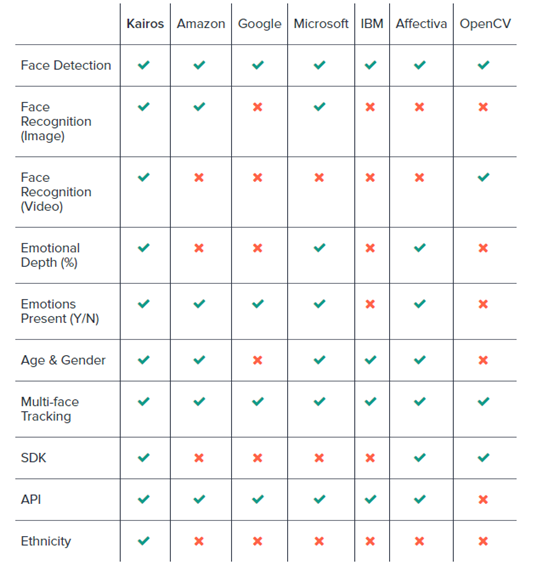
\includegraphics[scale=0.8]{uslugi_rozpoznawania.png}
	\caption{Przegląd usług rozpoznawania twarzy}
	\label{fig:picamera}
\end{figure}

\section{Open Cv}
OpenCv (Open Source Computer Vision Library) jest open sourcową biblioteką napisaną w języku C. Udostępniono liczne interfejsy biblioteki pozwalające na pracę z nią miedzy innymi w języku C++ i Python. Biblioteka wspiera systemy operacyjne Linux oraz Windows. Biblioteka została ukierunkowana na przetwarzanie obrazu w czasie rzeczywistym. W licznie udostępnionych funkcjach można znaleźć moduły pozwalające na detekcję i rozpoznawanie twarzy na obrazie, które zostały szerzej opisane w kolejnym punkcie.

\subsection{Detekcja twarzy}
Głównym wykrywaczem twarzy wykorzystywanym przez OpenCv jest kaskadowy klasyfikator Haar'a ale poza nim istnieją również inne metody. Jedną z nich jest wykorzystanie głębokiej sieci neuronowej.

\subsection{Rozpoznawanie twarzy}
\subsubsection{Eigenfaces} \label{eigen}
Eigenfaces, inaczej nazywany algorytmem twarzy własnych opiera się na metodzie analizy głównych składowych, która rozpoczyna się wyznaczeniem średniej wartości dla obrazów z tą samą etykietą identyfikującą daną osobę.
Weźmy $n$ wektorów $x_{i}$ powstałych jako reprezentacje obrazów przedstawiających daną twarz. Dla tych wektorów wyznaczona zostaje wartość średnia $\mu$.
$$
\mu=\frac{1}{n}\sum_{i=1}^{n}x_{i}
$$
Następnie dla każdego wektora $x_{i}$ wyznaczana jest różnica od wartości średniej $\mu$.
$$
\psi= x_{i}-\mu
$$
Na podstawie wartości $\psi_{i}$ wyznacza się macierz kowariancji $C$.
$$
C=\frac{1}{n}\sum_{i=1}^{n}\psi_{i}\psi_{i}^{T}
$$
Kolejnym krokiem jest wyznaczenie wartości $\lambda_{i}$ oraz $\nu_{i}$ tak by spełniony był warunek:
$$
C\nu_{i}=\lambda_{i}\nu_{i} \textrm{ dla $i=$1,2,...,n}
$$
Wartość $\lambda_{i}$ nazywana wartością własną amcierzy $C$, a odpowiadający jej wektor $\nu_{i}$ wektorem własnym $C$.
W przypadku algorytmu Eigenfaces branych jest pod uwagę $k$ głównych składowych $\lambda_{i}$, wyznaczonych na podstawie odrzucenia $n-k$ wartości najmniejszych. Dla każdego wektora wyznaczany jest wektor następujący:
$$
y_{i}=W^{T}(x_{i}-\mu) \textrm{ gdzie $W=(\nu_{1}, \nu_{2}, ..., \nu_{k})$}
$$
Identyfikacja twarzy algorytmem Eigenfaces polega na wykonaniu kroków:
\begin{enumerate}
\item Wartości głównych składowych zostają wyznaczone dla wszystkich obrazów uczących.
\item Wartość głównych składowych zostaje wyznaczona dla badanego zdjęcia
\item Dla obrazu wejściowego zostaje wyznaczony wektor najbliższy dla wartości obliczonych dla obrazów z bazy danych.
\end{enumerate}

\subsubsection{Fisherfaces} \label{fisher}
Algorytm Fisherfaces opiera się na liniowej analizie dyskryminacyjnej (LDA) i polega na wyznaczeniu wektora cech pozwalającego na rozdzielenie obiektów przynależnych do różnych klas. W przypadku problemu rozpoznawania twarzy, przez klasy obiektów rozumiane są zbiory obrazów przedstawiające tego samego użytkownika. Problem sprowadza się do wyznaczenia wektora, który stanowi przybliżoną granicę między dwiema klasami obiektów, jednak można go uogólnić do problemu wieloklasowego.
Wyznaczanie poszukiwanego wektora rozpoczyna się od wyznaczenia wartości średniej $\nu$ wszystkich obiektów znajdujących się w rozpatrywanym zbiorze, oraz wartości średniej $\nu_{i}$ wewnątrz poszczególnych klas. 
$$
\mu=\frac{1}{N}\sum_{i=1}^{N}x_{i}
$$
Gdzie $N$ oznacza liczebność rozpatrywanego zbioru $x_{i}$
$$
\mu_{i}=\frac{1}{|X_{i}|}\sum_{x_{j}eX_{i}}x_{j}
$$
Gdzie $X_{i}$ jest klasą obiektów o indeksie $i$, dla $i=1,2,...,n$ dla $n$ oznaczającego liczbę klas. Następnie wyznaczana jest macierz rozproszenia wewnątrzklasowego $S_{B}$ oraz macierz średniego rozproszenia wewnątrzklasowego $S_{W}$.
$$
S_{B}=\sum_{i=1}^{n}N_{i}(\mu-\mu_{i})(\mu-\mu_{i})^{T}
$$
$$
S_{W}=\sum_{i=1}^{n}\sum_{x_{j}eX_{i}}(x_{j}-\mu_{i})(x_{j}-\mu_{i})^{T}
$$
Rozwiązanie problemu sprowadza się do znalezienia danych, które pozwolą na otrzymanie największej wartości określającej stosunek rozproszenia wewnątrzklasowego do średniego wewnętrznego rozproszenia klas. Stąd algorytm poszukuje wektora $d$, dla którego poniższa funkcja osiąga maksimum.
$$
f(d)=\frac{d^{T}S_{B}d}{d^{T}S_{W}d}
$$
W celu zmniejszenia złożoności problemu, stosuje się modyfikację powyższego kryterium, wykorzystując macierz $W$ złożona z $k$ głównych wektorów własnych wyznaczonych dla macierzy kowariancji $C$ wszystkich elementów zbioru.
$$
f(d)=\frac{d^{T}W^{T}S_{B}d}{d^{T}S_{W}d}
$$
Znalezienie wektora $d$ pozwala na wyznaczenie optymalnego kierunku rozdzielającego dwie klasy obiektów.

\subsubsection{Local Binary Patterns Histograms} \label{lbph}
W odróżnieniu od holistycznego podejścia w dwóch poprzednich metodach, algorytm histogramów lokalnych binarnych wzorców wykorzystuje lokalne cechy przetwarzanych obiektów.
Dla każdego piksela wyznaczany jest ciąg binarny na podstawie porównania wartości z każdym z sąsiadów. W przypadku, gdy jego wartośc jest większa wtedy przyjmuje wartość 1, a 0 w przypadku przeciwnym. Stąd dla każdego piksela wyznaczana jest wartość $p$-znakowego binarnego ciągu, nazywanego lokalnym binarnym wzorcem.  Wyznaczanie można przeprowadzić w otoczeniu o dowolnym promieniu. W ogólności wartość funkcji LBP dla piksela o współrzędnych $(x_{c},y_{c})$ wyznacza się następująco: 
$$
LBP(x_{c},y_{c})=\sum_{p=0}^{p-1}2^{p}S(i_{p}-i_{c})
$$
Gdzie $p$ jest rozmiarem rozpatrywanego sąsiedztwa o środku w punkcie $(x_{c},y_{c})$ i jasności o wartości $i_{c}$, a $i_{n}$ jest wartością jasności dla $n$- tego punktu sąsiedztwa.
$S(x)$ jest funkcją znaku definiowaną następująco:
$$
S(x) = \left\{ \begin{array}{ll}
1 & \textrm{ dla $x>0$}\\
0 & \textrm{ w p.p.}
\end{array} \right.
$$
Działanie algorytmu polega na podzieleniu obrazu wejściowego na $m$ różnych części i wyznaczenia dla niego wartości LBP jasności pikseli. Następnie dla każdego regionu wyznaczany jest histogram wyliczonych wartości. Tak wyznaczone wartości są konkatenowane do postaci wektora.
Dla próbki wejściowej zostaje wyznaczony wektor histogramów, który następnie jest porównywany z wektorami obrazów użytych do uczenia sieci. Przewidywana etykieta jest wyznaczana na podstawie etykiety wektora najbliższego sąsiada.

\section{Azure Cognitive Services}
Cognitive Services jest częścią platformy Azure stworzonej przez Microsoft. Usługa jest standardowo płatna, ale w przypadku użytku na potrzeby studenckie przyznawany jest darmowy dostęp na ograniczony czas. Cognitive Services zajmuje się rozwiązywaniem problemów biznesowych dzięki sztucznej inteligencji. Do dostępnych modułów między innymi należą:
\begin{itemize}
\item obraz- algorytmy przetwarzania obrazów umożliwiające inteligentne identyfikowanie, podpisywanie i moderowanie grafik,
\item mowa- konwertowanie wypowiedzi audio na tekst, weryfikacja głosowa,
\item język- przetwarzanie języka naturalnego.
\end{itemize}
Na cele tego projektu wykorzystano moduł dotyczący przetwarzania obrazu, a dokładniej wykrywanie i rozpoznawanie twarzy w nim dostępne. Producent zadbał o prostą możliwość integracji z większością popularnych języków programistycznych poprzez udostępnienie paczek deweloperskich. W przypadku braku SDK dla wybranego języka istnieje możliwość skorzystania z udostępnionego REST Api. Na stronie producenta można znaleźć obszerną dokumentację oraz tutoriale.

\section{AWS Rekognition}
Usługa Rekognition jest odpowiednikiem Azure Cognitive Services ograniczonym do rozwiązań związanych z przetwarzaniem obrazu i video. Do wielu dostępnych funkcji należy analiza obrazu, detekcja twarzy i tekstu, porównywanie oraz rozpoznawanie twarzy. Dla wybranych języków programistycznych udostępniono SDK oraz obszerną dokumentację z licznymi przykładami kodu.
